\documentclass[aps,pre,twocolumn,floatfix]{revtex4-2}

\usepackage[T1]{fontenc}
\usepackage{amsmath,amssymb,amsfonts}
\usepackage{graphicx}
\usepackage{dcolumn}
\usepackage{bm}
\usepackage{booktabs}
\usepackage{microtype}
\usepackage{xcolor}
\usepackage[hidelinks]{hyperref}

\graphicspath{{../figures/}}
\renewcommand{\topfraction}{0.95}
\renewcommand{\bottomfraction}{0.95}
\renewcommand{\textfraction}{0.05}
\renewcommand{\floatpagefraction}{0.85}


\begin{document}

\title{Search-Budget Artifacts in Continuous Causal Emergence:\\Fixed-Step Riemannian Optimization Manufactures Apparent Scale Dependence}

\author{Felipe Mora}
\thanks{ORCID: 0009-0001-1034-5948}
\email{felipe.morar@usm.cl}
\affiliation{Departamento de Industrias, Universidad T\'ecnica Federico Santa Mar\'ia, Avenida Espa\~na 1680, Valpara\'iso, Chile}
\affiliation{Facultad de Ingenier\'ia, Negocios y Ciencias Agroambientales, Universidad Vi\~na del Mar, Vi\~na del Mar, Chile}

\date{\today}

\begin{abstract}
Continuous causal emergence quantifies macroscopic informational dominance in complex dynamical systems by maximizing an effective information objective over projection matrices on the Stiefel manifold. Here, we demonstrate that both the macro objective and its Riemannian gradient scale quadratically with the norm of the whitened transition operator. Consequently, first-order Riemannian optimization with a fixed step size violates the step length prescribed by Riemannian optimization theory and exhibits scale-dependent convergence: as the operator contracts, the manifold displacement per iteration collapses, leaving the optimizer trapped near initialization. In an empirical pipeline applied to industrial portfolio returns, this mechanism underestimates causal emergence by up to 103-fold, while corrupting the selected macro-dimension toward boundary scales. A single feasible projection that exceeds the reported optimum proves the reported value was not the maximum, without requiring any claim of global optimality. We show that established Riemannian line search, Barzilai-Borwein, and Cayley transform methods restore 100\% of an analytical ground truth without increasing the restart budget. Finally, we formulate a zero-cost diagnostic bracket consisting of a spectral upper bound and a feasible projection lower bound that reliably certifies optimizer convergence.
\end{abstract}

\maketitle

\section{Introduction}

Causal emergence formalizes the principle that a macroscopic description of a complex system can exhibit stronger causal efficacy than its microscopic constituent dynamics~\cite{Hoel2013,Hoel2017}. Originally formulated for discrete Markov chains via Shannon entropy coarse-graining~\cite{Rosas2020,Klein2020}, the framework was recently extended to continuous-state Gaussian stochastic processes~\cite{Liu2024,Liu2025,Yang2025}. In continuous formulations, causal emergence is quantified by effective information (EI), defined as the mutual information between an intervention distribution and the resulting system state. The macro-level representation is obtained by searching for a linear projection matrix $W$ constrained to the Stiefel manifold $\mathrm{St}(q, p) = \{W \in \mathbb{R}^{q \times p} : W W^T = I_q\}$, which maps a $p$-dimensional microscopic state to a $q$-dimensional macro state ($q < p$).

In discrete systems, finding an optimal grouping is a combinatorial partitioning problem. In continuous systems, evaluating causal emergence requires maximizing a non-concave objective over a smooth matrix manifold~\cite{Liu2024}. In continuous state-space models and in our audited pipeline, this maximization is conducted via first-order Riemannian gradient descent with a fixed learning rate and a fixed iteration budget (typically 100 iterations across 12 restarts). Recently, Yang et al.~\cite{Yang2025} introduced an alternative neural network framework (NIS+), reporting optimization traces across training epochs over five repeated trials (their Fig.~3b), and explicitly noting that ``if the training is insufficient, it may lead to incorrect identification of CE'' (p.~10). However, across this literature, numerical estimates are not compared against analytical ground truths or theoretical upper bounds, and sensitivity to the search budget has not been evaluated in a controlled manner.

In this paper, we show that first-order Riemannian gradient descent with a fixed step size harbors a severe, parameter-dependent artifact. Because the effective information objective and its Riemannian gradient both vanish quadratically with the norm of the whitened transition operator, the distance traversed across the manifold in a fixed number of iterations collapses whenever the operator contracts. As a result, whenever comparative studies sweep parameters that contract the transition operator (such as increasing regularization strength, decaying physical coupling, or decreasing sample size), the apparent variation in causal emergence is confounded with the scale-dependent convergence failure of the optimizer.

This paper makes four interconnected contributions:
(i) We show that the mechanism is a direct corollary of the Riemannian convergence theory of Boumal, Absil, and Cartis~\cite{Boumal2019,Boumal2019erratum}, identifying that in continuous causal emergence estimators, the pullback Lipschitz smoothness constant $L_g$ scales with the transition operator norm, aligning optimizer deficit with the parameter under study;
(ii) We formalize a zero-cost diagnostic bracket, bounding the true maximum between a spectral upper bound and an explicit feasible projection lower bound;
(iii) We quantify this deficit in our own empirical pipeline applied to industrial portfolio returns, demonstrating up to a 103-fold underestimation while corrupting the selected macro-dimension $q^*$;
(iv) We evaluate established Riemannian corrections (Armijo line search, Barzilai-Borwein step sizes, and Cayley transform retractions) and show that adaptive step scaling restores 100\% of an analytical ground truth without increasing the restart budget.

\section{Continuous Causal Emergence on the Stiefel Manifold}

Consider a discrete-time, linear stochastic continuous system governed by a first-order vector autoregressive process:
\begin{equation}
x_{t+1} = A x_t + \epsilon_{t+1}, \quad \epsilon_t \sim \mathcal{N}(0, \Sigma_\epsilon),
\label{eq:micro_var}
\end{equation}
where $x_t \in \mathbb{R}^p$, $A \in \mathbb{R}^{p \times p}$ is the transition matrix, and $\Sigma_\epsilon \in \mathbb{R}^{p \times p}$ is the positive-definite innovation covariance matrix. 

Following the interventionist definition of effective information introduced by Hoel et al.~\cite{Hoel2013,Hoel2017}, an intervention is imposed at time $t$ by setting $x_t \sim \mathcal{N}(0, \Sigma_{\mathrm{do}})$. To guarantee invariance under a common scalar rescaling of the state variables ($x_t \to c\, x_t$, under which $A$ is unchanged while $\Sigma_x$, $\Sigma_\epsilon$ and $\sigma_{\mathrm{do}}^2$ all scale by $c^2$), the intervention variance is calibrated to the mean observational variance:
\begin{equation}
\Sigma_{\mathrm{do}} = \sigma_{\mathrm{do}}^2 I_p, \quad \sigma_{\mathrm{do}}^2 = \kappa^2 \frac{\operatorname{tr}(\Sigma_x)}{p},
\label{eq:scale_invariant_do}
\end{equation}
where $\kappa > 0$ is a dimensionless parameter ($\kappa = 1$) and $\Sigma_x$ denotes the state covariance, well defined as the stationary Lyapunov covariance when $\rho(A) < 1$ and estimated as the empirical sample covariance over an observational window otherwise. This calibration does not confer invariance under a heterogeneous coordinatewise rescaling $x_t \to D x_t$ with $D$ diagonal, under which $A \to D A D^{-1}$. Under a Gaussian intervention, which maximizes differential entropy among continuous distributions with the prescribed covariance $\Sigma_{\mathrm{do}}$, the microscopic effective information evaluated through the linear Gaussian channel~\cite{Hoel2013,Hoel2017} is:
\begin{equation}
EI_p = \frac{1}{2} \left[ \ln\det(\sigma_{\mathrm{do}}^2 A A^T + \Sigma_\epsilon) - \ln\det(\Sigma_\epsilon) \right].
\label{eq:ei_micro}
\end{equation}

Continuous causal emergence in linear stochastic iteration systems was introduced by Liu, Yuan, and Zhang~\cite{Liu2024} using uniform hypercube interventions, and subsequently studied by Liu et al.~\cite{Liu2025} and Yang et al.~\cite{Yang2025}. The closed-form Gaussian channel evaluated here corresponds to the maximum-entropy Gaussian intervention model implemented in the audited pipeline.

A macroscopic model of dimension $q < p$ is obtained through an orthonormal projection matrix $W \in \mathrm{St}(q, p)$ satisfying $W W^T = I_q$. The audited estimator associates each such $W$ with a reduced linear Gaussian macro model defined by:
\begin{equation}
A_m = W A W^T, \quad \Sigma_m = W \Sigma_\epsilon W^T.
\label{eq:macro_matrices}
\end{equation}
We emphasize that the projected state $y_t = W x_t$ does not in general constitute an autonomous closed VAR(1) process, because
\begin{equation}
W x_{t+1} = W A W^T y_t + W A (I_p - W^T W) x_t + W \epsilon_{t+1},
\label{eq:closure_defect}
\end{equation}
and the residual term vanishes only under exact dynamical closure, $W A (I_p - W^T W) = 0$. Equation~(\ref{eq:macro_matrices}) therefore defines the Galerkin-type projected surrogate adopted by the audited estimator, not an exact marginal dynamics. The macroscopic effective information evaluated on this reduced model is:
\begin{equation}
f(W) = \frac{1}{2} \left[ \ln\det(\sigma_{\mathrm{do}}^2 A_m A_m^T + \Sigma_m) - \ln\det(\Sigma_m) \right].
\label{eq:macro_obj}
\end{equation}
The causal emergence density for a given dimension $q$ is defined as the difference in information densities:
\begin{equation}
\Delta J_q(W) = \frac{f(W)}{q} - \frac{EI_p}{p}.
\label{eq:delta_j}
\end{equation}
The continuous causal emergence of the system is the supremum over all admissible macro dimensions and orthonormal projections:
\begin{equation}
CE^* = \max_{1 \le q < p} \max_{W \in \mathrm{St}(q, p)} \Delta J_q(W).
\label{eq:cefi_def}
\end{equation}

\section{Mechanism: Quadratic Vanishing of Gradients and Theory of Step Sizing}

Evaluating Eq.~(\ref{eq:cefi_def}) requires maximizing $f(W)$ over $\mathrm{St}(q, p)$ for each candidate dimension $q$. We now establish the mechanism of scale-dependent convergence.

\subsection{Small-Operator Expansion}

Let $M = \sigma_{\mathrm{do}}^2 A_m A_m^T + \Sigma_m$. Factoring out $\Sigma_m^{1/2}$ yields:
\begin{equation}
f(W) = \frac{1}{2} \ln\det\left( I_q + \sigma_{\mathrm{do}}^2 \Sigma_m^{-1} A_m A_m^T \right).
\label{eq:obj_det_form}
\end{equation}
Consider a family of transition operators parameterized by a contraction factor $\alpha > 0$, such that $A(\alpha) = \alpha A_0$. As $\alpha \to 0$, the matrix $X = \sigma_{\mathrm{do}}^2 \Sigma_m^{-1} A_m A_m^T$ satisfies $\|X\| = \mathcal{O}(\alpha^2)$. Using the series expansion $\ln\det(I + X) = \operatorname{tr}(X) - \frac{1}{2}\operatorname{tr}(X^2) + \dots$, we obtain the leading-order expansion:
\begin{equation}
\begin{split}
f(W) &= \frac{\sigma_{\mathrm{do}}^2}{2} \operatorname{tr}\left( \Sigma_m^{-1} A_m A_m^T \right) + \mathcal{O}(\|A\|^4) \\
&= \frac{\sigma_{\mathrm{do}}^2}{2} \operatorname{tr}\big( (W \Sigma_\epsilon W^T)^{-1} (W A W^T) \\
&\quad \times (W A^T W^T) \big) + \mathcal{O}(\|A\|^4).
\end{split}
\label{eq:taylor_expansion}
\end{equation}
Thus, the objective $f(W)$ scales quadratically with the transition operator: $f(W) = \mathcal{O}(\|A\|^2)$.

\subsection{Riemannian Gradient Scaling}

To compute the gradient on the Stiefel manifold~\cite{Edelman1998,Absil2008}, we first evaluate the Euclidean gradient in $\mathbb{R}^{q \times p}$. Differentiating Eq.~(\ref{eq:macro_obj}) with respect to $A_m$ and $\Sigma_m$ yields:
\begin{align}
P &= \frac{\partial f}{\partial A_m} = \sigma_{\mathrm{do}}^2 M^{-1} A_m, \label{eq:P_deriv} \\
Q &= \frac{\partial f}{\partial \Sigma_m} = \frac{1}{2} \left( M^{-1} - \Sigma_m^{-1} \right). \label{eq:Q_deriv}
\end{align}
Because $M = \Sigma_m + \mathcal{O}(\alpha^2)$, we have $M^{-1} = \Sigma_m^{-1} + \mathcal{O}(\alpha^2)$, from which $P = \sigma_{\mathrm{do}}^2 \Sigma_m^{-1} A_m + \mathcal{O}(\alpha^3) = \mathcal{O}(\alpha)$. For $Q$, the resolvent identity gives:
\begin{equation}
Q = -\frac{\sigma_{\mathrm{do}}^2}{2} \Sigma_m^{-1} A_m A_m^T \Sigma_m^{-1} + \mathcal{O}(\alpha^4) = \mathcal{O}(\alpha^2).
\end{equation}
Applying the chain rule to $W$ produces the Euclidean gradient:
\begin{equation}
\nabla_W f(W) = \left( P W A^T + P^T W A \right) + \left( Q W \Sigma_\epsilon + Q^T W \Sigma_\epsilon \right).
\label{eq:euclidean_grad}
\end{equation}
Both terms scale as $\mathcal{O}(\alpha^2)$, so $\| \nabla_W f(W) \| = \mathcal{O}(\|A\|^2)$.

Under the embedded Euclidean (Frobenius) metric on the Stiefel manifold $\langle \xi, \eta \rangle = \operatorname{tr}(\xi \eta^T)$, the Riemannian gradient $\operatorname{grad}_{\mathrm{St}} f(W)$ is the orthogonal projection of $\nabla_W f(W)$ onto the tangent space $T_W \mathrm{St}(q, p) = \{ \xi \in \mathbb{R}^{q \times p} : \xi W^T + W \xi^T = 0 \}$~\cite{Edelman1998,Absil2008}:
\begin{equation}
\operatorname{grad}_{\mathrm{St}} f(W) = \nabla_W f(W) - \operatorname{sym}\!\left( \nabla_W f(W) W^T \right) W,
\label{eq:riemannian_grad_general}
\end{equation}
where $\operatorname{sym}(X) = \frac{1}{2}(X + X^T)$. Because $f(W)$ is strictly invariant under macroscopic coordinate rotations $W \mapsto R W$ for any $R \in \mathrm{O}(q)$, differentiating along the infinitesimal gauge transformation $R = I_q + \varepsilon \Omega$ with $\Omega = -\Omega^T$ gives $\operatorname{tr}\!\left( \Omega \left( \nabla_W f(W) W^T \right)^T \right) = 0$ for every skew-symmetric $\Omega$. Hence $\nabla_W f(W) W^T$ is identically symmetric and $\operatorname{sym}(\nabla_W f(W) W^T) W = W (\nabla_W f(W))^T W$, so that Eq.~(\ref{eq:riemannian_grad_general}) reduces to the form implemented in the audited pipeline:
\begin{equation}
\operatorname{grad}_{\mathrm{St}} f(W) = \nabla_W f(W) - W (\nabla_W f(W))^T W.
\label{eq:riemannian_grad}
\end{equation}
Because the tangent projection is an orthogonal linear operator with unit norm, the Riemannian gradient inherits the exact quadratic scaling:
\begin{equation}
\| \operatorname{grad}_{\mathrm{St}} f(W) \| = \mathcal{O}(\|A\|^2).
\label{eq:riemannian_grad_scaling}
\end{equation}

\subsection{Connection to Riemannian Smoothness Theory}

In the non-convex Riemannian optimization theory of Boumal, Absil, and Cartis~\cite{Boumal2019,Boumal2019erratum}, Theorem~2.8 establishes that if the pullback $f \circ \mathcal{R}_W$ has Lipschitz-continuous gradient with constant $L_g$ on tangent balls of radius $\varrho$, then Riemannian gradient descent run with the certified step size
\begin{equation}
\gamma_k = \min\!\left( \frac{1}{L_g}, \frac{\varrho}{\|\operatorname{grad}_{\mathrm{St}} f(W_k)\|} \right)
\label{eq:prescribed_step}
\end{equation}
returns an approximate stationary point in at most $\lceil 2 (f(W_0) - f^*) L_g / \epsilon^2 \rceil$ iterations, provided $\epsilon \le \varrho L_g$. Adapting the sign convention to our maximization problem ($F = -f$), reaching $\|\operatorname{grad}_{\mathrm{St}} f(W)\| \le \epsilon$ requires at most
\begin{equation}
N(\epsilon) \le \left\lceil \frac{2 \left[ f^* - f(W_0) \right] L_g}{\epsilon^2} \right\rceil
\label{eq:iteration_bound}
\end{equation}
iterations, where $f^* = \max_{W \in \mathrm{St}(q,p)} f(W)$ and $f^* - f(W_0) \ge 0$. Whenever the gradient norm is small relative to $\varrho L_g$, the first branch is active and the certified step reduces to $1/L_g$, which is the regime relevant to the contracted operators studied below.

Write $A(t) = t A_0$ for the contracted family. Using the uniform small-operator expansion of the reduced objective, together with the smoothness of the retraction and the compactness of $\mathrm{St}(q, p)$, there exist constants $C > 0$, $\varrho > 0$ and $t_0 > 0$ such that
\begin{equation}
\sup_{\substack{W \in \mathrm{St}(q, p) \\ \|\xi\| \le \varrho}} \left\| D^2 (f_t \circ \mathcal{R}_W)(\xi) \right\|_{\mathrm{op}} \le C t^2, \qquad 0 < t \le t_0,
\label{eq:pullback_hessian_bound}
\end{equation}
whether $\sigma_{\mathrm{do}}^2$ is held fixed or recalibrated through the stationary state covariance $\Sigma_x(t) = \Sigma_\epsilon + \mathcal{O}(t^2)$. This certifies the admissible smoothness constant $\bar{L}_g(t) = C t^2 = \mathcal{O}(t^2)$, so that the certified step scale satisfies $\gamma_k(t) = \Theta(t^{-2})$: as the operator contracts, traversing a fixed distance on the manifold requires a step size growing inversely with the squared operator norm.

In the audited production pipeline, however, updates are executed via QR retraction with a constant step size $\eta = 0.05$:
\begin{equation}
W_{k+1} = \mathcal{R}\left( W_k + \eta \operatorname{grad}_{\mathrm{St}} f(W_k) \right).
\label{eq:qr_retract}
\end{equation}
The ratio between the implemented step and the certified theoretical scale therefore collapses quadratically, $\eta / \gamma_k(t) = \mathcal{O}(t^2) \to 0$, so a fixed step becomes asymptotically far more conservative than the theory prescribes. Over a budget of $K = 100$ iterations, the cumulative displacement measured in the ambient Frobenius norm satisfies
\begin{equation}
\begin{split}
\| W_K - W_0 \|_F &\le \sum_{k=0}^{K-1} \| W_{k+1} - W_k \|_F \\
&= \mathcal{O}(K \eta \|A\|^2).
\end{split}
\label{eq:trajectory_bound}
\end{equation}
As $\|A\| \to 0$ we obtain $\| W_K - W_0 \|_F \to 0$, and because $\mathrm{St}(q, p)$ is a compact embedded submanifold, convergence in the ambient Frobenius metric implies convergence in the manifold topology, $d_{\mathrm{St}}(W_K, W_0) \to 0$. The iterate is therefore trapped in an infinitesimal neighborhood of its initialization $W_0$. The failure mode is not numerical instability or oscillation, but asymptotic stagnation.

\subsection{Analytical Invariance of Scale Normalization}

The preceding derivation yields an analytical statement that small-operator problems are not intrinsically harder to optimize. Under the contraction $A(t) = t A_0$, the suboptimality gap satisfies $\Delta f(t) = f_t^* - f_t(W_0) = \mathcal{O}(t^2)$ while $\bar{L}_g(t) = C t^2$. Evaluating stationarity relative to the natural scale of the objective, that is, setting the relative gradient tolerance $\epsilon(t) = t^2 \epsilon_0$, the admissibility condition $\epsilon(t) \le \varrho \bar{L}_g(t)$ reduces to $\epsilon_0 \le \varrho C$, which is independent of $t$. For any fixed relative tolerance $\epsilon_0$ satisfying that condition,
\begin{equation}
N(t) \le \frac{2 \, \mathcal{O}(t^2) \, (C t^2)}{\left[ t^2 \epsilon_0 \right]^2} = \mathcal{O}(1) \quad \text{as } t \to 0.
\label{eq:complexity_invariant}
\end{equation}
The worst-case stationarity complexity therefore remains bounded under operator contraction once the step size and the stopping tolerance are matched to the natural scale of the objective. The observed scale-dependent stagnation is attributable to step-size mismatch rather than to any intrinsic divergence of stationarity complexity.

\begin{figure}[!t]
\centering
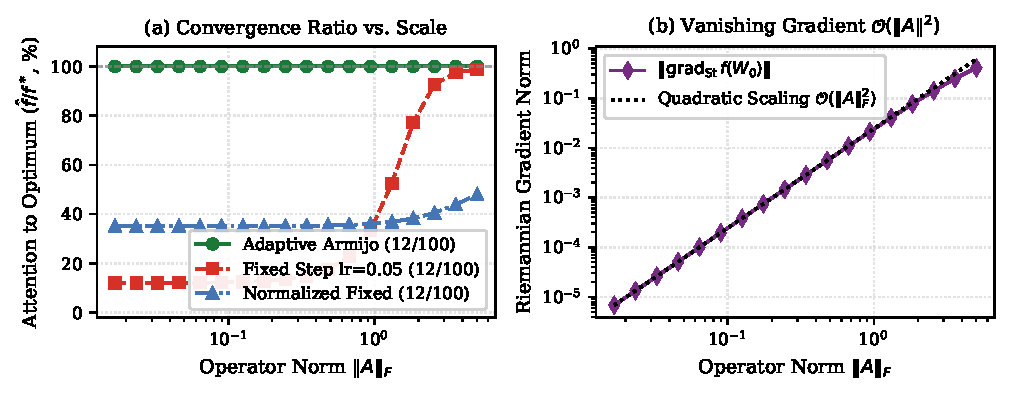
\includegraphics[width=\columnwidth]{fig1_operator_scaling.pdf}
\caption{(a) Attention to the true analytical optimum ($\hat{f} / f^*$, \%) as a function of operator Frobenius norm $\|A\|_F$ across 18 scales. The fixed-step optimizer (red squares) collapses below $\|A\|_F \approx 1.5$, reaching 12.08\% at $\|A\|_F = 0.017$. Adaptive Armijo line search (green circles) achieves 100.00\% across all scales. The normalized fixed-step control (blue triangles) holds its attention ratio constant across scales (35.15\%), illustrating that normalization removes the scale dependence of Eq.~(\ref{eq:complexity_invariant}) even though a fixed step remains suboptimal at any single scale. (b) Norm of initial Riemannian gradient $\|\operatorname{grad}_{\mathrm{St}} f(W_0)\|$ strictly follows theoretical quadratic scaling $\mathcal{O}(\|A\|_F^2)$ (dotted line).}
\label{fig:scaling}
\end{figure}

\section{Zero-Cost Diagnostic Brackets}

Because $f(W)$ is non-concave on $\mathrm{St}(q, p)$, certifying global optimality is generally intractable. However, certifying optimizer failure does not require knowing the global optimum. We introduce a zero-cost diagnostic bracket consisting of a spectral upper bound and a feasible projection lower bound.

\subsection{Proposition 1: Spectral Upper Bound via Singular Value Contraction}

\textbf{Proposition 1.} \emph{Let $A \in \mathbb{R}^{p \times p}$ and let $\Sigma_\epsilon \succ 0$ be a symmetric positive-definite innovation covariance with minimum eigenvalue $\lambda_{\min}(\Sigma_\epsilon) > 0$. For any macro dimension $q < p$ and any $W \in \mathrm{St}(q, p)$, the macroscopic effective information of the reduced Gaussian model satisfies}
\begin{equation}
f(W) \le \frac{1}{2} \sum_{i=1}^q \ln\left( 1 + \frac{\sigma_{\mathrm{do}}^2}{\lambda_{\min}(\Sigma_\epsilon)} s_i(A)^2 \right),
\label{eq:spectral_bound_general}
\end{equation}
\emph{where $s_1(A) \ge s_2(A) \ge \dots \ge s_p(A)$ are the singular values of $A$. Under isotropic noise $\Sigma_\epsilon = \sigma_\epsilon^2 I_p$ the bound specializes to}
\begin{equation}
f(W) \le \frac{1}{2} \sum_{i=1}^q \ln\left( 1 + \frac{\sigma_{\mathrm{do}}^2}{\sigma_\epsilon^2} s_i(A)^2 \right).
\label{eq:spectral_bound}
\end{equation}

\emph{Proof.} Write $S_W = W \Sigma_\epsilon W^T$. Factoring $S_W$ out of Eq.~(\ref{eq:macro_obj}) gives
\begin{equation}
f(W) = \frac{1}{2} \sum_{i=1}^q \ln\left( 1 + \sigma_{\mathrm{do}}^2 \, s_i\!\left( S_W^{-1/2} W A W^T \right)^2 \right).
\label{eq:f_singular_form}
\end{equation}
For any unit vector $u \in \mathbb{R}^q$, the vector $v = W^T u$ satisfies $\|v\|_2^2 = u^T W W^T u = 1$ by the Stiefel constraint, so the Rayleigh-Ritz theorem gives $u^T S_W u = v^T \Sigma_\epsilon v \ge \lambda_{\min}(\Sigma_\epsilon) > 0$ and hence $\lambda_{\min}(S_W) \ge \lambda_{\min}(\Sigma_\epsilon)$, that is, $\| S_W^{-1/2} \|_2 \le \lambda_{\min}(\Sigma_\epsilon)^{-1/2}$. Using $s_i(XY) \le \|X\|_2 \, s_i(Y)$ and the fact that $W A W^T$ is an orthonormal compression of $A$, for which singular-value contraction under orthogonal compression gives $s_i(W A W^T) \le s_i(A)$~\cite{Thompson1972,HornJohnson2013}, we obtain
\begin{equation}
s_i\!\left( S_W^{-1/2} W A W^T \right) \le \frac{s_i(A)}{\sqrt{\lambda_{\min}(\Sigma_\epsilon)}}, \quad i = 1, \dots, q.
\label{eq:interlacing}
\end{equation}
Since $x \mapsto \frac{1}{2}\ln(1 + c x^2)$ is strictly increasing on $[0, \infty)$ for $c > 0$, substituting Eq.~(\ref{eq:interlacing}) into Eq.~(\ref{eq:f_singular_form}) yields Eq.~(\ref{eq:spectral_bound_general}); setting $\lambda_{\min}(\Sigma_\epsilon) = \sigma_\epsilon^2$ yields Eq.~(\ref{eq:spectral_bound}). $\blacksquare$

Equation~(\ref{eq:spectral_bound_general}) is a closed-form, fully analytic bound that requires only the singular values of $A$ and the smallest eigenvalue of $\Sigma_\epsilon$, and it holds for anisotropic innovation covariance without any whitening approximation.

\subsection{Proposition 2: Exact Ground Truth for Symmetric Systems}

\textbf{Proposition 2.} \emph{When $A$ is symmetric ($A = A^T$) and $\Sigma_\epsilon = I_p$, the bound in Eq.~(\ref{eq:spectral_bound}) is attained with equality by taking $W^* \in \mathrm{St}(q, p)$ to be the eigenvectors associated with the $q$ largest absolute eigenvalues $|\lambda_i(A)| = s_i(A)$.}

\emph{Proof.} Let $A = V \Lambda V^T$ with $|\lambda_1| \ge |\lambda_2| \ge \dots \ge |\lambda_p|$. Choosing $W^* = V_{:, 1:q}^T$ gives $W^* (W^*)^T = I_q$, $S_{W^*} = I_q$ and $W^* A (W^*)^T = \operatorname{diag}(\lambda_1, \dots, \lambda_q)$, whose singular values are $|\lambda_i| = s_i(A)$ for $i = 1, \dots, q$. Equality holds identically in Eq.~(\ref{eq:interlacing}), providing an exact analytical ground truth. $\blacksquare$

\subsection{Proposition 3: Feasible Projection Certificate}

\textbf{Proposition 3.} \emph{Let $\hat{f}_{\mathrm{rep}}$ be a reported numerical estimate of the maximum macro effective information. For any orthonormal matrix $W_{\mathrm{wit}} \in \mathrm{St}(q, p)$, if $f(W_{\mathrm{wit}}) > \hat{f}_{\mathrm{rep}}$, then $\hat{f}_{\mathrm{rep}}$ is sub-optimal.}

\emph{Proof.} By definition of the supremum, $f^* = \sup_{W \in \mathrm{St}} f(W) \ge f(W_{\mathrm{wit}})$. If $f(W_{\mathrm{wit}}) > \hat{f}_{\mathrm{rep}}$, then $f^* > \hat{f}_{\mathrm{rep}}$, proving that $\hat{f}_{\mathrm{rep}}$ failed to achieve the maximum without requiring knowledge of $f^*$. $\blacksquare$

\begin{figure}[!t]
\centering
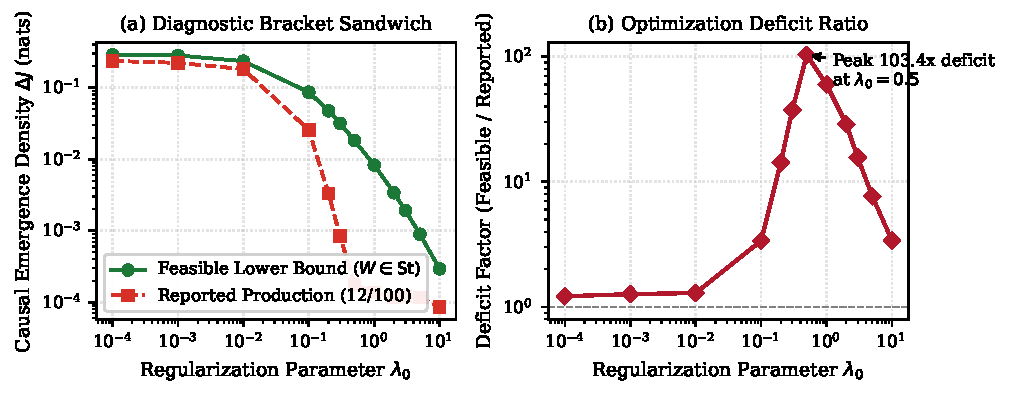
\includegraphics[width=\columnwidth]{fig2_diagnostic_bracket.pdf}
\caption{(a) Zero-cost diagnostic bracket applied across an empirical regularization trajectory ($\lambda_0 \in [10^{-4}, 10]$) on industrial portfolio returns ($p=30$, 18 non-overlapping windows). The feasible projection lower bound (green circles) exceeds the production estimate (red squares). (b) The optimization deficit factor (feasible lower bound divided by reported estimate) rises from $1.2\times$ at weak regularization to a peak of $103.4\times$ at $\lambda_0 = 0.5$.}
\label{fig:bracket}
\end{figure}

\section{Empirical and Synthetic Demonstrations}

\subsection{Benchmark on Known Analytical Ground Truth}

We evaluate the fixed-step production optimizer and Riemannian corrections against the exact analytical optimum of Proposition~2 ($p=30, \Sigma_\epsilon = I_p$). As reported in Table~\ref{tab:benchmarks}, the fixed-step production configuration with budget 12/100 (12 restarts, 100 iterations, $\eta = 0.05$) reaches 88.94\% of the analytical optimum. A smaller budget configuration (4/35) achieves 44.15\% and selects an incorrect dimension ($q^* = 2$ instead of $q^*=1$).

An expanded budget of 25/150 (treated as a numerical ceiling in previous pipeline checks) requires 6.572~s and 108,750 steps, yet remains 5.69\% below the optimum (94.31\%). In contrast, standard Riemannian methods that automatically adjust step size achieve 100.00\% of the analytical optimum with the same 12 restarts: adaptive Armijo line search~\cite{Boumal2019} in 3.389~s, Riemannian Barzilai-Borwein (RBB)~\cite{Iannazzo2018} in 3.710~s, and the Wen-Yin Cayley transform method~\cite{WenYin2013} in 3.387~s. This confirms that the deficit is caused by fixed step sizing rather than an insufficient restart count.

\begin{table}[!t]
\caption{Benchmark of manifold optimizers on a symmetric system ($p=30$) with known analytical optimum ($CE^* = 0.178174, q^* = 1$). All algorithms executed from identical random seeds. The estimate, the selected dimension, the attained fraction of the optimum and the step count are deterministic and reproduce exactly; wall-clock times were measured on a single machine and are indicative only.}
\label{tab:benchmarks}
\begin{ruledtabular}
\footnotesize
\setlength{\tabcolsep}{2pt}
\begin{tabular*}{\columnwidth}{@{\extracolsep{\fill}}lcccccc@{}}
Method & Budget & CEFI & $q^*$ & \% Opt & Deficit & Time (s) \\
\hline
Fixed Step & 4/35 & 0.078668 & 2 & 44.15\% & 55.85\% & 0.251 \\
Fixed Step & 12/100 & 0.158463 & 1 & 88.94\% & 11.06\% & 2.133 \\
Fixed Step & 25/150 & 0.168031 & 1 & 94.31\% & 5.69\% & 6.572 \\
Adaptive Armijo & 12/100 & 0.178174 & 1 & 100.00\% & 0.00\% & 3.389 \\
Riemannian BB & 12/100 & 0.178174 & 1 & 100.00\% & 0.00\% & 3.710 \\
Wen-Yin Cayley & 12/100 & 0.178174 & 1 & 100.00\% & 0.00\% & 3.387 \\
\end{tabular*}
\end{ruledtabular}
\end{table}

\subsection{Characterizing the Scaling Law and Breakdown Point}

In Fig.~\ref{fig:scaling}(a), we map the attention ratio ($\hat{f} / f^*$) as a function of operator norm $\|A\|_F$ across 18 logarithmically spaced scales. At large operator norms ($\|A\|_F = 5.03$), the fixed-step optimizer reaches 98.82\% of the optimum. As $\|A\|_F$ contracts, performance drops monotonically: it crosses 52.52\% at $\|A\|_F = 1.31$, and reaches 12.08\% at $\|A\|_F = 0.017$. Over the same range, adaptive Armijo line search maintains 100.00\% attention across all scales.

Fig.~\ref{fig:scaling}(b) plots the norm of the initial Riemannian gradient, verifying that $\|\operatorname{grad}_{\mathrm{St}} f(W_0)\|$ follows the quadratic scaling $\mathcal{O}(\|A\|_F^2)$ derived in Eq.~(\ref{eq:riemannian_grad_scaling}).

When $A$ is normalized by its Frobenius norm prior to fixed-step optimization and evaluated at true scale, the attention ratio remains constant at 35.15\% across small scales (blue line in Fig.~\ref{fig:scaling}(a)). Normalization thus removes the scale dependence predicted by Eq.~(\ref{eq:complexity_invariant}), while the residual gap to the optimum reflects the fact that a fixed step of $\eta = 0.05$ is not the certified step $1/\bar{L}_g$ at the normalized scale either.

\begin{figure}[!t]
\centering
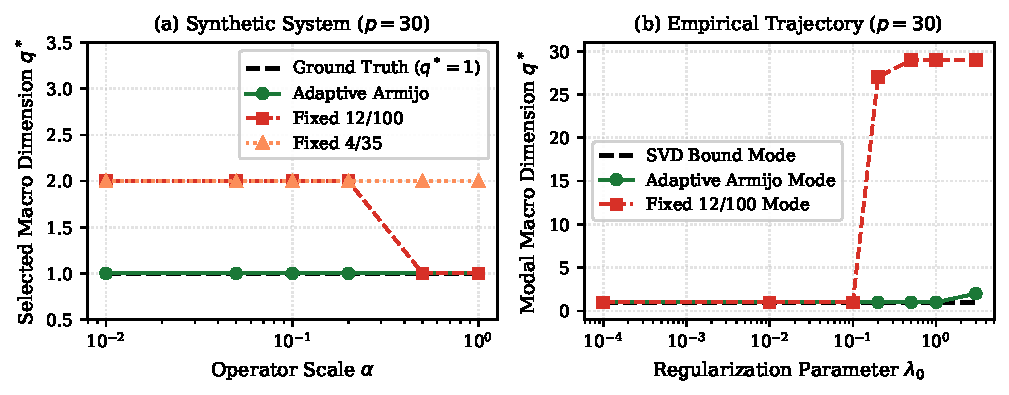
\includegraphics[width=\columnwidth]{fig3_dimension_corruption.pdf}
\caption{Corruption of selected macro-dimension $q^*$. (a) In the synthetic symmetric system ($q^*_{\mathrm{true}} = 1$), Fixed 4/35 selects $q^* = 2$ across all scales, and Fixed 12/100 switches to $q^* = 2$ when $\alpha \le 0.2$, whereas Adaptive Armijo preserves $q^* = 1$ everywhere. (b) Across 18 empirical portfolio return windows ($p=30$), increasing ridge regularization $\lambda_0$ causes the modal $q^*$ of Fixed 12/100 to jump from $q^* = 1$ to $q^* = 27$ ($\lambda_0 = 0.2$) and collapse to the micro boundary $q^* = 29$ ($\lambda_0 \ge 0.5$). The SVD bound and Adaptive Armijo confirm the true modal scale is $q^* \le 2$.}
\label{fig:q_corruption}
\end{figure}

\subsection{Deficit on Real Empirical Data: 103x Gap}

We evaluate the diagnostic bracket on an empirical continuous causal emergence pipeline applied to daily returns of 30 industry portfolios ($p=30$) over 18 non-overlapping 500-day windows, swept across ridge regularization parameters $\lambda_0 \in [10^{-4}, 10]$. Ridge regularization shrinks the estimated VAR(1) transition matrix $A$, inducing operator contraction.

As shown in Fig.~\ref{fig:bracket}(a), the production values (12/100) drop from $\Delta J = 0.236$ at $\lambda_0 = 10^{-4}$ to $0.000176$ at $\lambda_0 = 0.5$. However, evaluating admissible projection matrices $W \in \mathrm{St}(1, p)$ obtained from adaptive line search yields $\Delta J = 0.018208$ at $\lambda_0 = 0.5$. In Fig.~\ref{fig:bracket}(b), the ratio between the feasible lower bound and the production estimate reaches a peak deficit of $103.4\times$ at $\lambda_0 = 0.5$ (and exceeds $14\times$ across $\lambda_0 \in [0.2, 3.0]$). Because each witness projection satisfies $W W^T = I_1$, this proves that the trajectory produced by the fixed-step optimizer was dominated by optimizer stagnation.

\begin{figure}[!t]
\centering
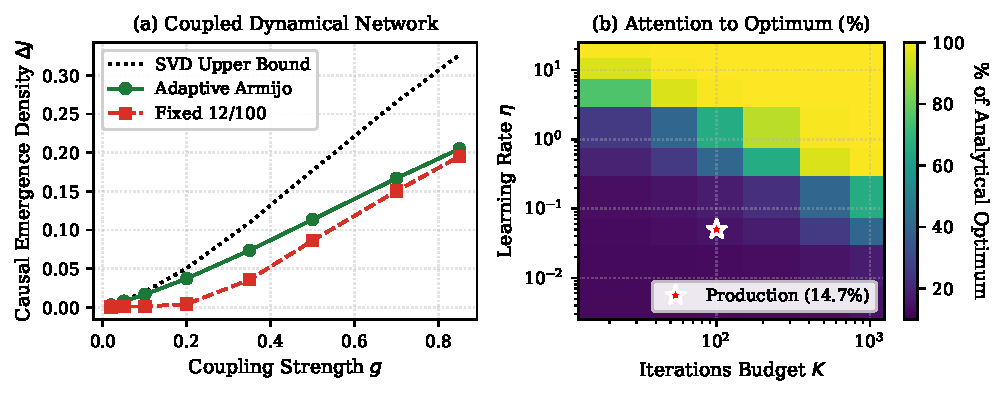
\includegraphics[width=\columnwidth]{fig4_generalization_and_grid.pdf}
\caption{Generalization and parameter disentanglement. (a) Synthetic directed network ($p=20$) sweeping physical coupling strength $g \in [0.02, 0.85]$. Weak coupling contracts the operator, causing Fixed 12/100 (red squares) to capture only 6.10\% of emergence at $g=0.10$, manufacturing an artificial threshold. Adaptive search (green circles) tracks the spectral profile. (b) Phase diagram of attention to optimum (\%) sweeping learning rate $\eta$ and iteration budget $K$ at contracted scale ($\alpha = 0.10$). Within a budget of $K \le 100$, reaching $>95\%$ with fixed steps requires scaling $\eta \ge 5.0$, whereas expanding iterations $K$ at production $\eta = 0.05$ (red star) reaches only 39.4\% at $K=1000$.}
\label{fig:generalization}
\end{figure}

\subsection{Corruption of the Selected Macro-Dimension}

In continuous causal emergence, the optimal macro scale $q^*$ is determined by identifying the peak of the emergence spectrum $\Delta J_q$. When the optimizer stagnates, the objective profile across $q$ flattens, and numerical noise dominates the argmax.

Fig.~\ref{fig:q_corruption}(a) demonstrates this on the synthetic system: while the ground truth is $q^* = 1$, Fixed 4/35 selects $q^* = 2$ everywhere, and Fixed 12/100 selects $q^* = 2$ when $\alpha \le 0.2$. In the empirical portfolio dataset [Fig.~\ref{fig:q_corruption}(b)], under weak regularization ($\lambda_0 = 10^{-4}$), every window selects $q^* \le 4$ with modal dimension 1, and 94.4\% still do at $\lambda_0 = 10^{-2}$. As regularization contracts the operator, the modal $q^*$ of Fixed 12/100 jumps to 27 at $\lambda_0 = 0.2$, and collapses to 29 (the micro boundary $p-1$) for $\lambda_0 \ge 0.5$ (where 0.0\% of windows have $q^* \le 4$). In contrast, both the SVD bound and the Adaptive Armijo optimizer identify $q^* = 1$ as the dominant modal scale across the entire regularization range. Thus, search-budget collapse manufactures both false scale dependence and spurious high-dimensional macro dynamics.

\subsection{Generalization Beyond Finance}

To verify that this failure is general to dynamical systems, we evaluated two non-financial benchmarks.

First, we modeled a synthetic network of 20 interacting continuous linear units with variable coupling strength $g \in [0.02, 0.85]$: $A(g) = 0.15 I_{20} + g C$, where $C$ is a normalized directed network adjacency matrix. As shown in Fig.~\ref{fig:generalization}(a), weak physical coupling contracts the transition operator. Under Fixed 12/100, the emergence estimate captures only 6.10\% of the spectral bound at $g = 0.10$ and 17.03\% at $g = 0.02$. The resulting fixed-step curve manufactures an artificial sigmoidal threshold that mimics a dynamical phase transition. In contrast, Adaptive Armijo captures $82.10\%$ of the bound at $g = 0.10$, where the fixed-step estimate collapses to $6.10\%$, and stays between $62.79\%$ and $95.87\%$ across the full coupling range, demonstrating that the apparent threshold is an optimization artifact.

Second, we systematically disentangled learning rate $\eta$ from iteration budget $K$ at a contracted scale ($\alpha = 0.10$, $\|A\|_F \approx 0.34$). As shown in Fig.~\ref{fig:generalization}(b), increasing the iteration budget from $K=100$ to $K=1000$ at the production learning rate ($\eta = 0.05$) only increases attention from 14.67\% to 39.40\%. In contrast, increasing the learning rate to match the $\mathcal{O}(\|A\|^{-2})$ curvature recovers the optimum almost immediately: at $\eta = 10.0$ the attention reaches $94.98\%$ at $K = 25$ and $98.99\%$ at $K = 50$, exceeding $99\%$ by $K = 100$, and at $\eta = 5.0$ the same thresholds are reached one grid step later.

Finally, we evaluated 793 monthly records of 10 primary climate oscillation indices from NOAA (including SOI, NAO, PDO, AO, and AMO). Under regularization ($\lambda_0 = 5.0, \|A\|_F = 0.32$), the deficit was $1.15\times$, compared to $103.4\times$ in portfolio returns ($p=30$). This comparison highlights the role of ambient manifold dimension: on $\mathrm{St}(1, 10)$, the tangent space has 9 dimensions, whereas on $\mathrm{St}(1, 30)$, it has 29 dimensions. Higher ambient dimension compounds the stagnation problem, reducing the probability that an iterate with collapsed step length makes progress.

\section{Discussion and Reporting Protocols}

In Riemannian optimization theory, convergence rates of gradient descent depend directly on the Lipschitz smoothness constants of the objective pullbacks~\cite{Boumal2019}. The key finding of this paper is not that fixed-step descent is scale-dependent, but that in continuous causal emergence estimators, this smoothness constant scales with the transition operator norm, which is precisely the variable swept across comparative studies. Whether sweeping ridge regularization, window length, or physical coupling strength, the parameter under study modulates the convergence rate of the optimizer, confounding methodological convergence with physical dynamics.

Furthermore, adaptive line search on Stiefel manifolds is thoroughly established in numerical optimization~\cite{Boumal2019,Iannazzo2018,Oviedo2021,Francisco2012,WenYin2013}. Theorem~2.11 of Boumal et al.~\cite{Boumal2019} proves that Armijo backtracking achieves the optimal iteration complexity bound without requiring knowledge of $L_g$. The persistence of fixed-step optimization in continuous causal emergence reflects a disconnect between numerical optimization theory and complex systems practice.

Selecting the maximum over candidate dimensions $q$ additionally introduces a selection bias analogous to the optimizer's curse~\cite{SmithWinkler2006}, in which maximum statistics systematically exceed their expected values under noise. Quantifying finite-sample biases in information-theoretic estimators has a long precedent in this journal~\cite{Wolpert1995,Holmes2019}; the search-budget collapse documented here shows that in continuous state spaces numerical optimization can introduce parameter-dependent artifacts that rival statistical sample effects. Multiple reported applications of continuous causal emergence share this vulnerable structure~\cite{HoelLevin2020,Tolle2026,ZhangLiu2023,HouDai2026}, whenever transition operators are estimated from data and swept across contracting parameter regimes under a fixed optimization budget.

To address this in future studies, we recommend a three-point reporting protocol: (i)~\textbf{Report the Zero-Cost Diagnostic Bracket:} publish the triplet $(\Delta J_{\mathrm{feas}}, \Delta J_{\mathrm{opt}}, \Delta J_{\mathrm{SVD}})$; if $\Delta J_{\mathrm{opt}} < \Delta J_{\mathrm{feas}}$, the estimate is certified sub-optimal; (ii)~\textbf{Employ Adaptive Step Sizing:} adopt adaptive Armijo backtracking, Barzilai-Borwein step selection, or Cayley retractions with best-iterate tracking; and (iii)~\textbf{Verify Scale Invariance via Normalization Controls:} when sweeping parameters that contract the operator, verify that scale-normalized controls produce consistent emergence profiles.

\section*{Data and Code Availability}

% TODO before submission: replace XXXXXXX with the Zenodo DOI minted from the
% GitHub release, and REPLACE_ME with the GitHub account name.
All code, figures and manuscript sources needed to regenerate every number, table and figure reported here are openly available at \url{https://doi.org/10.5281/zenodo.XXXXXXX}. The daily industry portfolio returns are obtained from the Kenneth R. French Data Library, whose contents are the property of Ken French and Dimensional Fund Advisors, and are therefore not redistributed; the repository provides a retrieval script that reconstructs the file used here from the original source and verifies it by checksum. All empirical results reported here use the vintage retrieved on 14 September 2026; because that library is periodically restated as the underlying data are revised, the script reports any deviation from that vintage rather than failing silently. The monthly climate oscillation indices are from the U.S. National Oceanic and Atmospheric Administration.

The repository additionally contains a Lean~4 development, machine-checked against \textsc{mathlib} and free of unproved assumptions, that formally verifies two of the statements made above. The first is the exact decomposition of the projected one-step map, Eq.~(\ref{eq:closure_defect}), strengthened to an equivalence: the projected state is an autonomous linear system for every initial condition if and only if $W A (I_p - W^T W) = 0$. The second is the Rayleigh-Ritz step of Proposition~1, established in the quadratic-form order and therefore in a form more general than the eigenvalue statement used in the proof. The singular-value contraction half of Proposition~1 is not formalized.

\begin{acknowledgments}
Computational evaluations were conducted using Python, NumPy, SciPy, and Matplotlib.
\end{acknowledgments}

\bibliography{referencias_paper1}

\end{document}
